\subsection{Risoluzione delle criticità}

\setLayout{vertical}

\begin{frame}
    \frametitle{Risoluzione delle criticità\footnote{Per una trattazione più dettagliata, si rimanda alla sezione "Risoluzione delle criticità" del Final Design Report.}}
    Abbiamo analizzato approfonditamente l'interfaccia originale, valutandovi linee guida riconosciute e facendola testare a giornalisti. 
    \begin{figure}
        \centering
        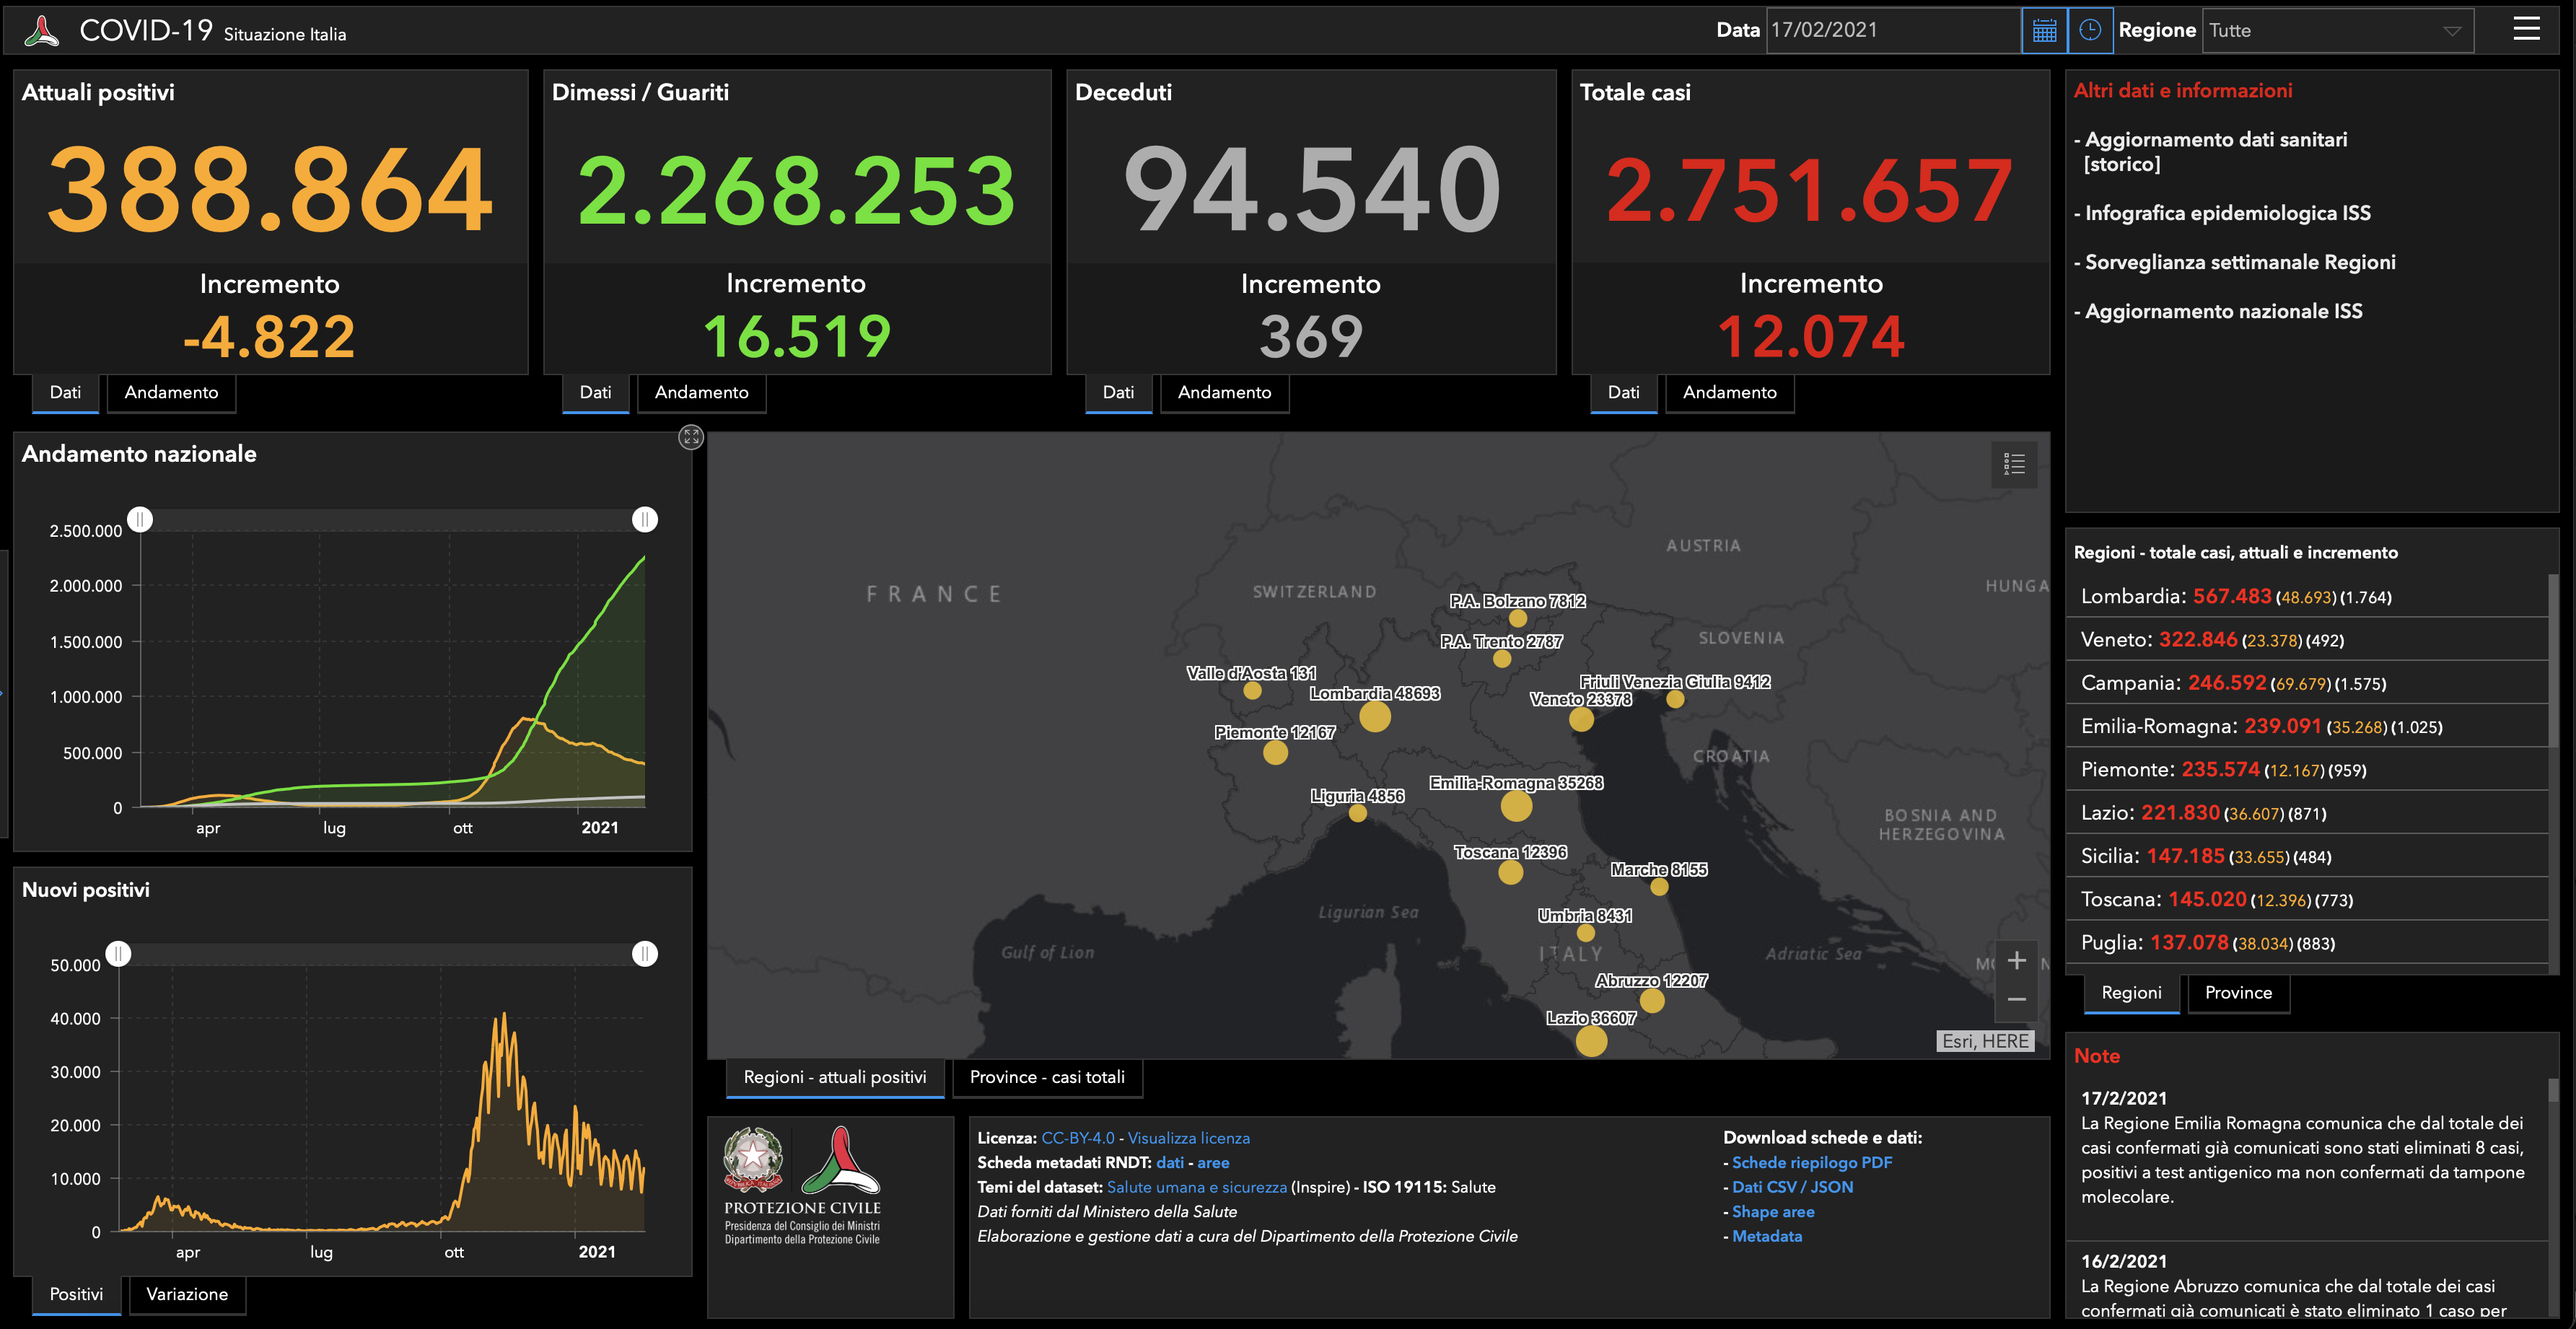
\includegraphics[width=.55\textwidth]{screen-interfaccia/screenshot-dashboard-DPC.png}
        \caption{Screenshot della dashboard del Dipartimento della Protezione Civile catturato il 17 febbraio '21.}
    \end{figure}
\end{frame}

\begin{frame}
    \frametitle{Risoluzione delle criticità}
    Abbiamo individuato le seguenti criticità: 
    \begin{itemize}
        \item<1-> \hyperlink{f:scarsa-leggibilita}{scarsa leggibilità per scritte piccole e riempimento disomogeneo;}        
        \item<2-> \hyperlink{f:mappa}{interazione con la mappa limitata e distante dalle aspettative degli utenti;}
        \item<3-> \hyperlink{f:significante}{discrepanza tra significante\footnote{Il \textit{significante} è una proprietà di un oggetto che ne rende visibile o ne esplicita l'affordance.} e comportamento effettivo;}
        \item<4-> \hyperlink{f:errori}{assenza di meccanismi di prevenzione degli errori nel widget calendario;}
        \item<5-> \hyperlink{f:grafica}{assenza di componenti grafiche per ridurre carico cognitivo;}
        \item<6-> \hyperlink{f:colore}{adozione del colore come unico mezzo distintivo delle componenti;}
        \item<7-> \hyperlink{f:difficolta}{difficoltà dell'interazione coi grafici.}
    \end{itemize}    

\end{frame}

\begin{frame}
    \label{f:scarsa-leggibilita}
    \frametitle{Scarsa leggibilità}    
    Soluzioni adottate: 
    \begin{itemize}
        \item<1-> abbiamo ingrandito la dimensione delle scritte particolarmente piccole e uniformato le dimensioni di tutte le componenti testuali in base alla loro importanza;
        \item<2-> abbiamo evitato la creazione di spazi vuoti, distribuendo tutti gli elementi in maniera omogenea sull'interfaccia;
        \begin{itemize}
            \item<2-> un esempio è la riprogettazione della componente delle note e quelle dei provvedimenti, per le quali abbiamo cambiato il semplice box dell'interfaccia originale in una sidebar on-demand, riuscendo a dare maggiore spazio e leggibilità, senza sacrificare in maniera permanente lo spazio dell'interfaccia.
        \end{itemize}
    \end{itemize}    

\end{frame}

\begin{frame}
    \frametitle{Scarsa leggibilità}
    \begin{figure}
        \centering
        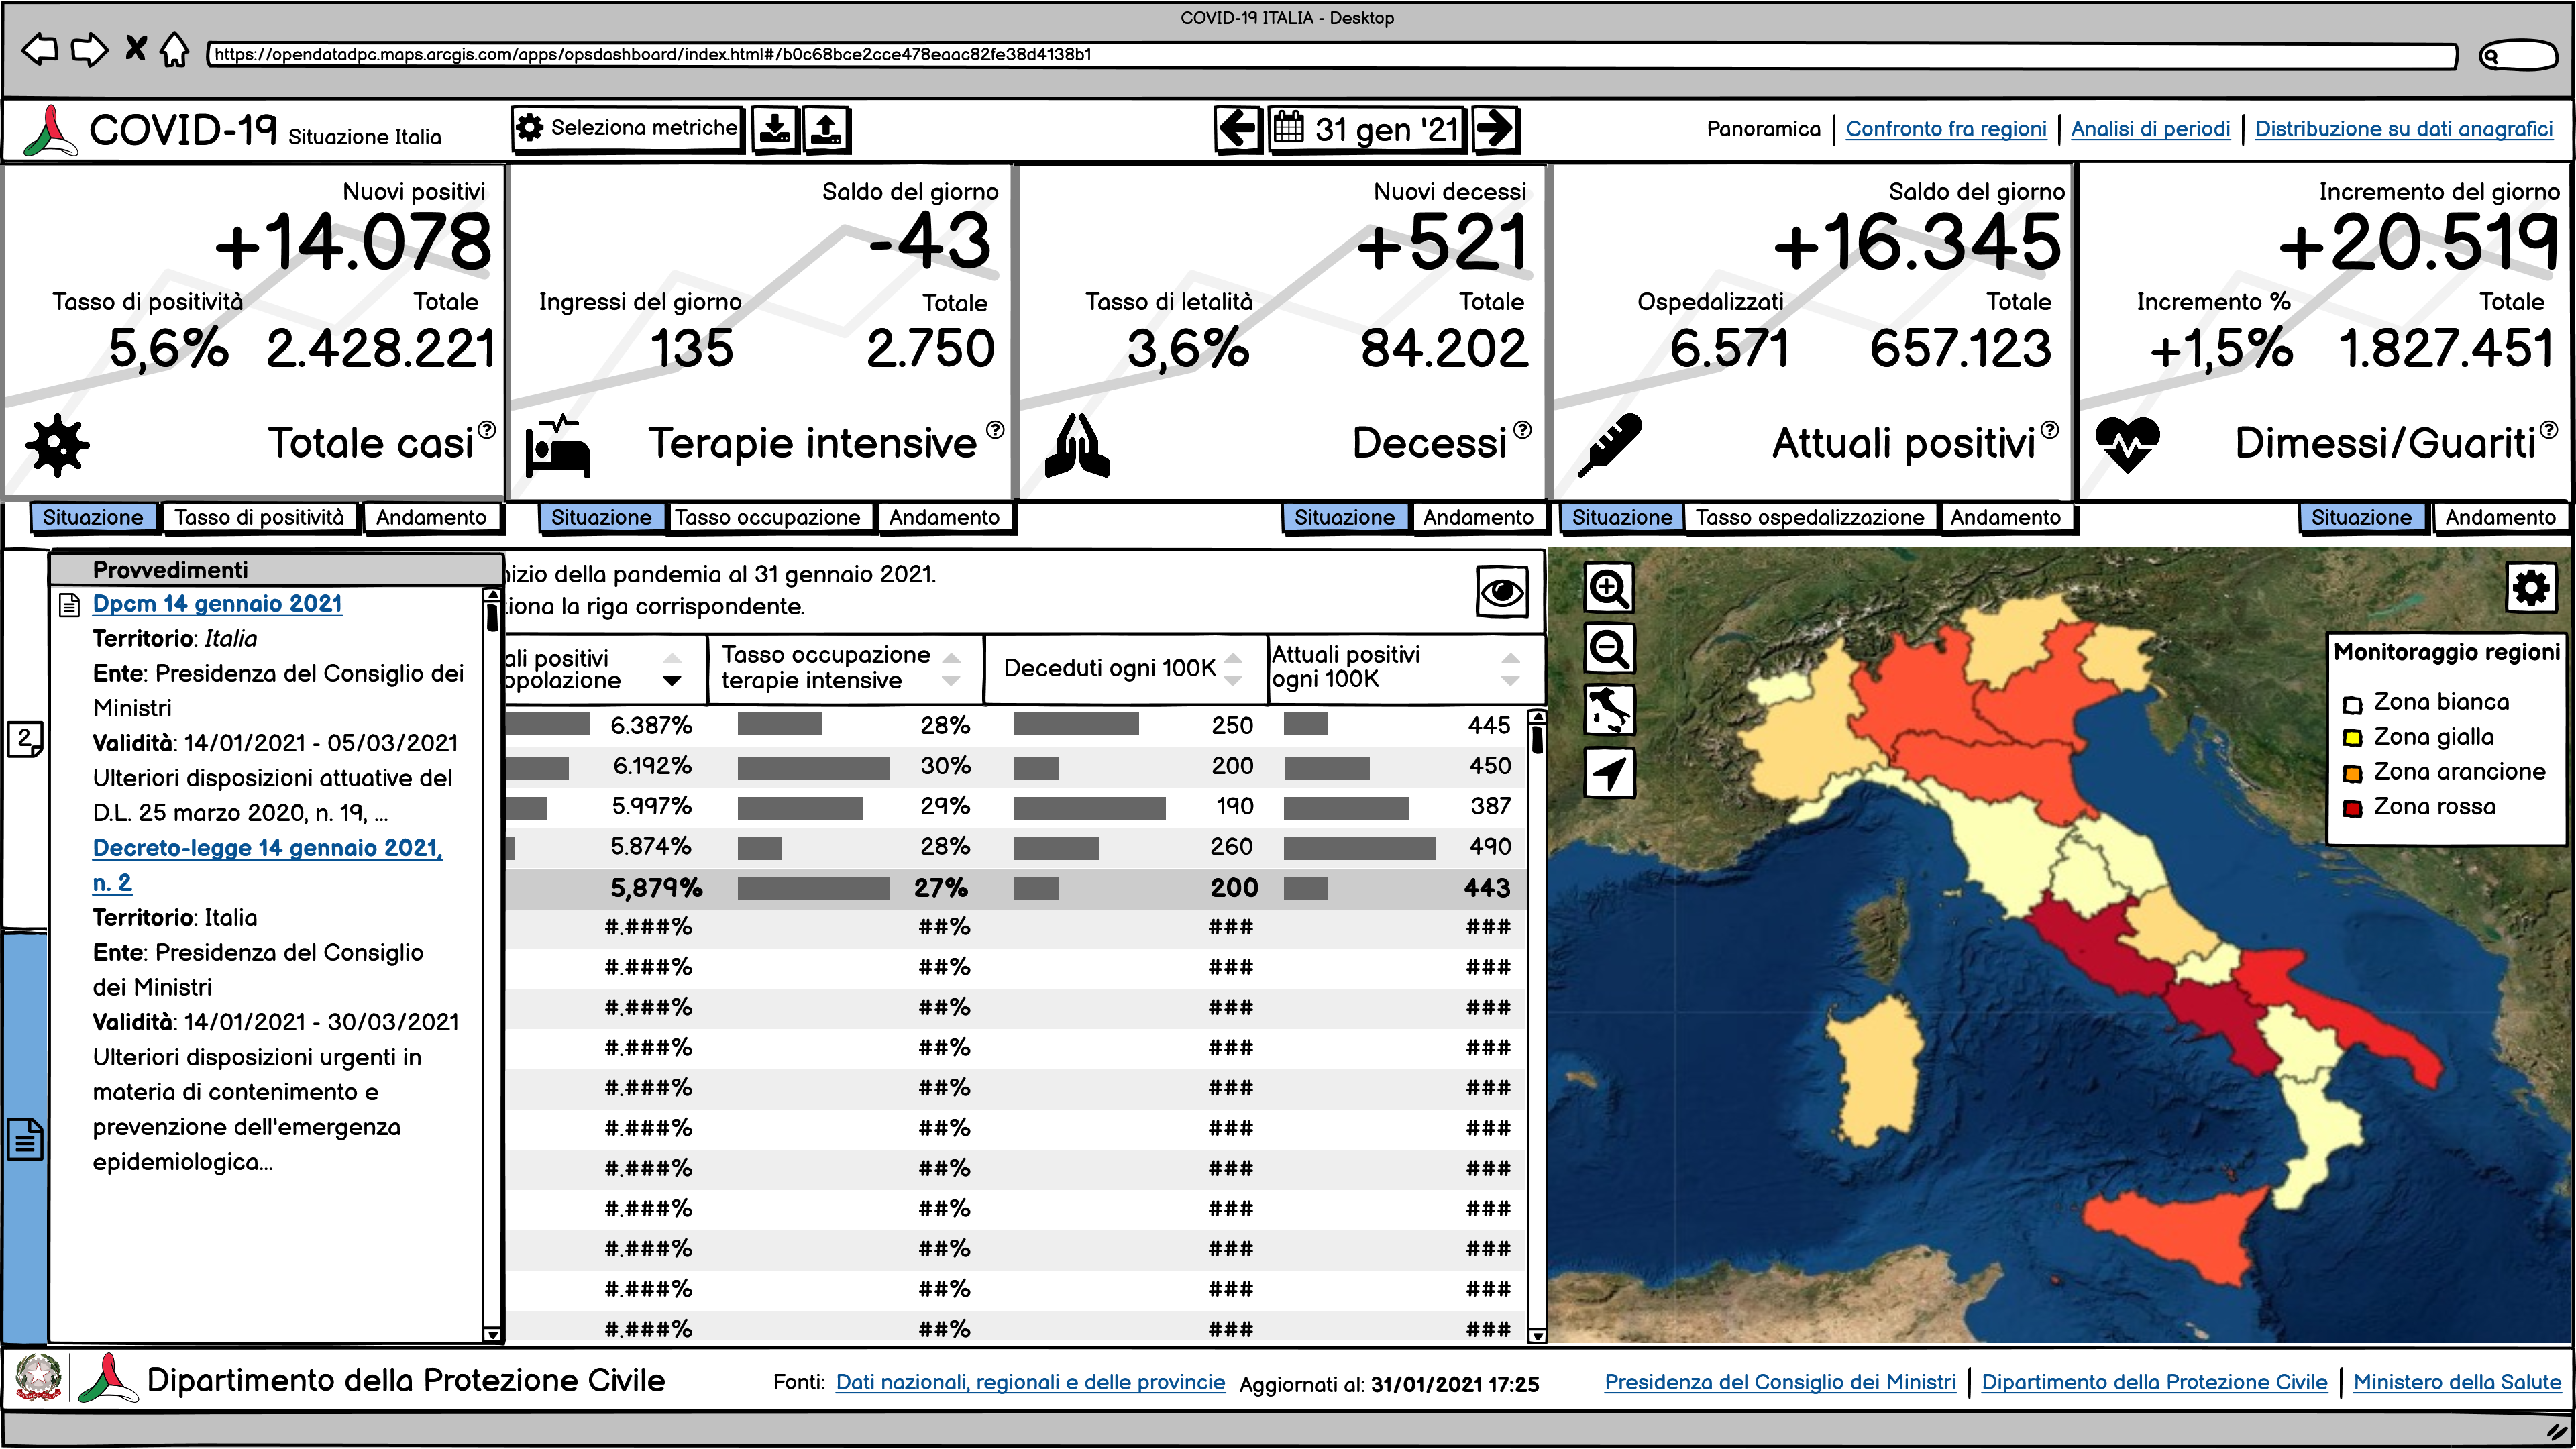
\includegraphics[trim = 0 20 0 55, clip, width=.85\textwidth]{screen-interfaccia/11 - Panoramica.png}
        \caption{Schermata "Panoramica" della nuova interfaccia con la sezione "Provvedimenti" aperta.}
    \end{figure}
\end{frame}

\begin{frame}
    \frametitle{Interazione mappa e modello mentale utenti}
    \label{f:mappa}
    Soluzioni adottate: 
    \begin{itemize}
        \item abbiamo cambiato la natura della mappa da bubble a heat map:
        \begin{itemize}
            \item ciò semplifica al giornalista la selezione di una certa regione: è sufficiente che clicchi sull'area corrispondente;
        \end{itemize}
    \end{itemize}
    \hspace{-8pt}
    \begin{tabular}{p{0.6\textwidth}p{0.4\textwidth}}    
        \begin{itemize}
            \item abbiamo aggiunto nuove funzionalità alla mappa, sotto forma di bottoni al cui clic l'utente può resettare il livello di zoom a quello di default o centrare la porzione visualizzata sulla sua posizione effettiva mediante geolocalizzazione.
        \end{itemize} &
            
        \begin{figure}
            \centering
            \vspace{-20pt}
            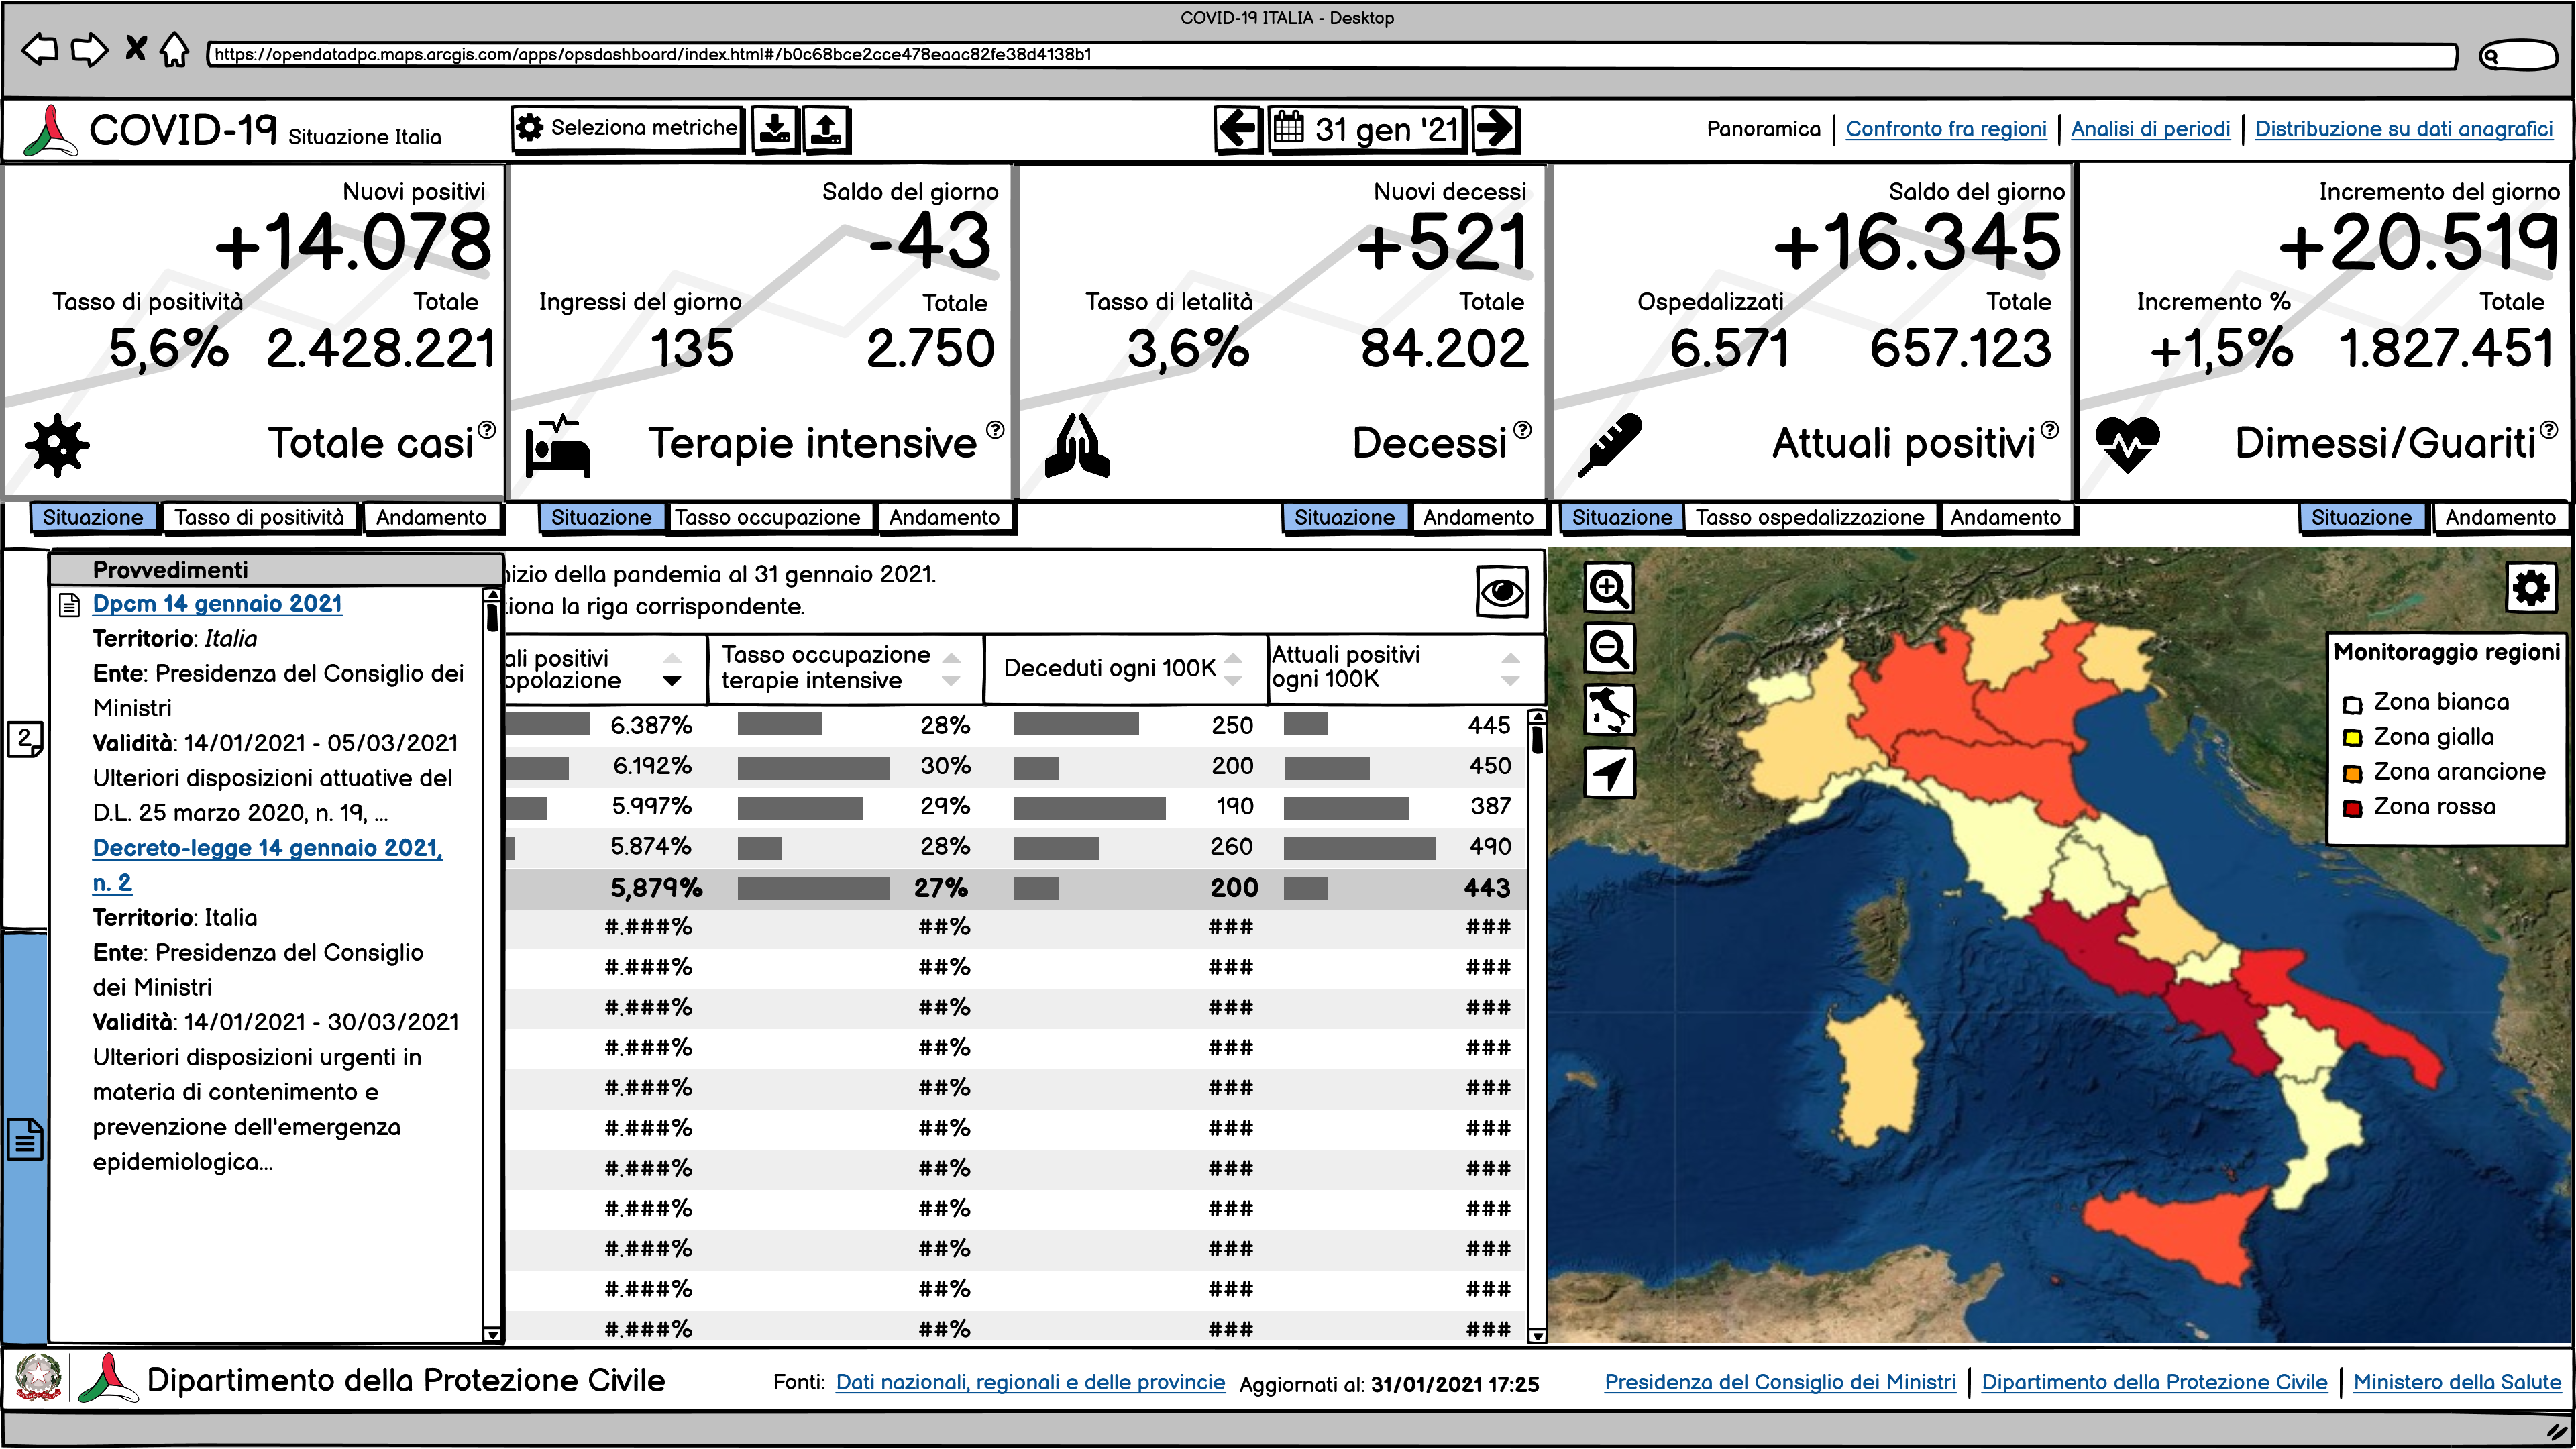
\includegraphics[trim = 880 60 0 310, clip, width=140pt]{screen-interfaccia/11 - Panoramica.png}
            \caption{Mappa di "Panoramica".}
        \end{figure} \\

    \end{tabular}   

\end{frame}


\begin{frame}
    \frametitle{Significante e comportamento effettivo}
    \label{f:significante}
    Per disambiguare ogni possibile interazione:
    \begin{itemize}
        \item<1-> abbiamo caratterizzato chiaramente i bottoni e al loro click seguono sempre azioni e/o feedback inequivocabili;
        \item<2-> abbiamo settato il mouse-over alla mappa e alle tabelle così che sia chiara la loro natura interattiva;
    \end{itemize}
\end{frame}

\begin{frame}
    \frametitle{Errori e calendario}
    \label{f:errori}
    Abbiamo migliorato l'usabilità del widget calendario, nonché adottati alcuni accorgimenti per prevenire o ridurre errori accidentali del giornalista; esempi:
    \begin{itemize}
        \item date successive al giorno corrente disabilitate\footnote{A livello di wireframe, non è possibile settare come disabilitate le date successive.}, impedendo al giornalista di selezionare così date per cui la dashboard non visualizzerebbe valori;
    \end{itemize}
    \hspace{-8pt}
    \begin{tabular}{p{0.6\textwidth}p{0.4\textwidth}}    
        \begin{itemize}
            \item aggiunta di bottoni tramite cui l'utente può agevolmente andare al giorno successivo o precedente a quello selezionato o, ancora, resettare la selezione alla data corrente; 
        \end{itemize} &
            
        \begin{figure}
            \centering
            \vspace{-10pt}
            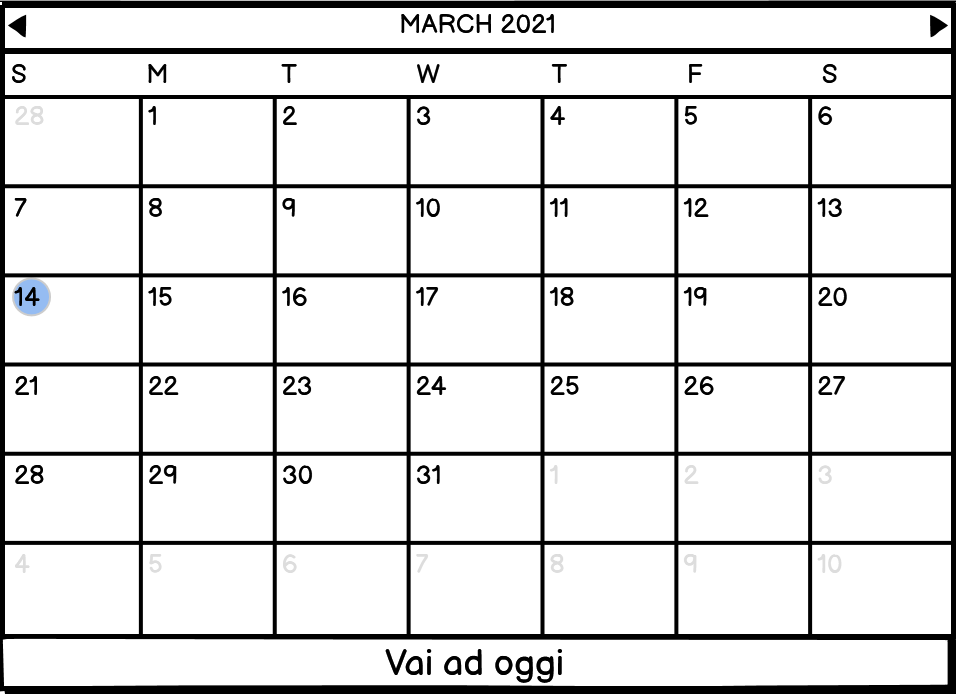
\includegraphics[width=85pt]{screen-interfaccia/calendar.png}
            \caption{Calendario aperto in "Panoramica".} 
        \end{figure}  \\
    \end{tabular}   
    
\end{frame}

\begin{frame}
    \frametitle{Componenti grafiche e carico cognitivo}
    \label{f:grafica}
    Trasversalmente alle schermate dell'interfaccia riprogettata, abbiamo aggiunto icone al fine di ridurre il carico cognitivo richiesto al giornalista per individuare e distinguere le varie componenti informative; esempi sono:
    \begin{itemize}
        \item icone dei box numerici;
        \item icone dei pulsanti;
        \item grafici a linea temporale;
        \item areogrammi;
        \item grafici a barre.
    \end{itemize}
\end{frame}

\begin{frame}
    \frametitle{Colore per distinguere componenti}
    \label{f:colore}
    Abbiamo ridotto l'utilizzo del colore come elemento distintivo delle componenti, affiancandolo sempre ad almeno un ausilio addizionale. Per esempio:
    \begin{itemize}
        \item il diverso tratto delle curve dei grafici;
        \item sottolineatura dei link.
    \end{itemize}
\end{frame}

\begin{frame}
    \frametitle{Difficoltà nell'interazione coi grafici}
    \label{f:difficolta}
    Abbiamo semplificato l'interazione coi grafici, facendo sì che al movimento del cursore corrisponda una proiezione sull'asse delle $x$ che intercetti le curve: 
    \begin{tabular}{p{0.6\textwidth}p{0.4\textwidth}}    
        \begin{itemize}
            \item in questa maniera, il giornalista può ottenere i dati puntuali, in maniera semplice, ponendo il cursore in un qualsiasi punto soprastante o sottostante a quello di suo interesse;
        \end{itemize} &
            
        \begin{figure}
            \centering
            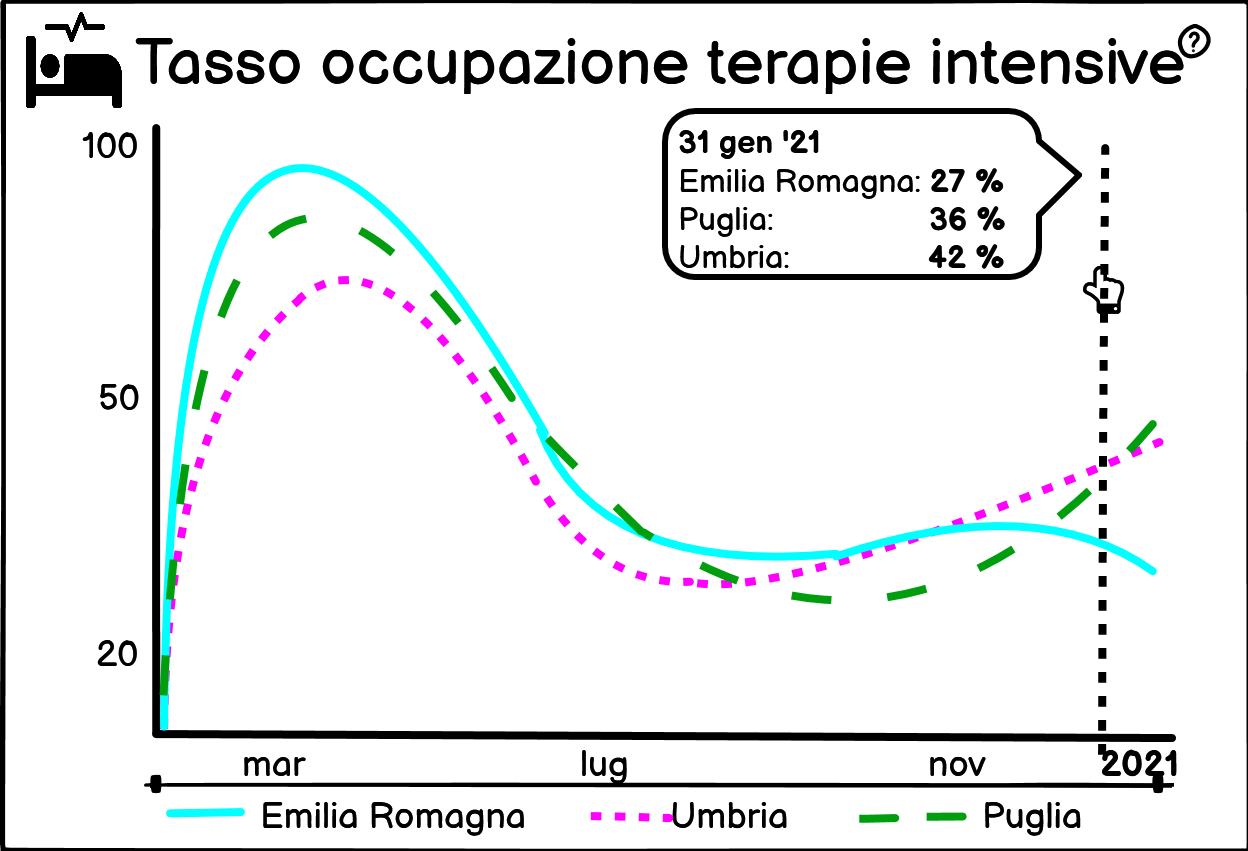
\includegraphics[width=150pt]{screen-interfaccia/graf.png}
            \caption{Grafico in "Confronto tra regioni".} 
        \end{figure}  \\
    \end{tabular}   
\end{frame}